

%per fare una lista codice spiegazione
%\begin{itemize}
%\item Spiegazione del codice
%\begin{verbatim}
%inserire qui il codice
%i rientri a capo si fanno premendo solo invio
%senza le due sbarrette //
%il testo verrà formattato esattamente così com'è
%\end{verbatim} 

\begin{itemize}

\item Inserimento nuovo utente (in media 2 volte al giorno)

\begin{verbatim}
insert into utente (
username, nome, cognome,indirizzo,
carCredito,password, email)
values (?);
\end{verbatim} 

\item Inserimento nuovo personaggio (in media 5 volte al giorno)

\begin{verbatim}insert into personaggio(
nome, razza, classe, livello, esperienza, soldi,
capelli, colorePelle, barba, volto, puntiVita, puniMana, attacco,
difesa, forza, destrezza, intelligenza, xPos, yPos, zPos)
values (?); 

\end{verbatim}
\item Inserimento nuovo NPC (in media 175 volta ogni 3 anni)

\begin{verbatim}

/* se NPC è amichevole */
insert into NPCAmichevole (
nome, livello, puntiVita, attacco, difesa, xPos, yPos, zPos) 
values(...);

/* se NPC è ostile */

insert into NPCOstlie (
codNPCOst, nome, livello, puntiVita, attacco,
difesa, ricompensaOro, ricompensaExp, xPos, yPos, zPos)

values(...);
\end{verbatim}

\item Inserimento nuovo oggetto (in media 200 volte ogni 3 anni)

\begin{verbatim}

	insert into oggetto  (nome, descrizione) values(...);

	/* se l'oggetto è un equipaggiamento */
	
	insert into Equipaggiamento (
	nome, livello,	tipo, peso, attacco,
	difesa, forza, destrezza, intelligenza,
	prezzoVendita, prezzoAcquisto) 
	values (?);

	/* se l'oggetto è un consumabile */
	
	insert into Consumabili (
	nome, livello, puntiVita, puntiMana, attacco,
	difesa, forza, destrezza, 	intelligenza,
	durata,prezzoVendita, prezzoAcquisto) 
	values (?);


	/* se l'oggetto è un oggetto missione */
	insert into OggettiMissione(nome)
	 values (?);

\end{verbatim}
\item Inserimento nuova missione (in media 100 volte ogni 3 anni)

\begin{verbatim}
	insert into missione Missione(
	codMiss, nome, descrizione, livello, completamento,
	ricompensaOro, ricompensaExp, ricompensaOgg, xMiss,
	yMiss, zMiss)
	values( ?);
	
	/* se la missione  prevede l'uccisione di NPC */
	
	insert into ObiettivoAnimato(missione, nemico,
	obiettivo, contatore) values(...);
	
	/* se la missione prevede il recupero di oggetti*/
	
	insert into ObiettivoInanimato(missione, oggMiss,
	obiettivo, contatore) values (?);

\end{verbatim}

\item Inserimento missione intrapresa (in media 35000 volte al giorno)
\begin{verbatim}

insert into Intraprendenza(personaggio, missione)
values(...);
\end{verbatim}

\item Inserimento missione completata (in media 21000 volte al giorno)

\begin{verbatim}

insert into Completamento (personaggio, missione)
values(...);

\end{verbatim}

\item Inserimento nuova abilità (in media 10 volte ogni 3 anni)

\begin{verbatim}

insert into Abilità (nome, descrizione, classe, livello,
costoMana,  attacco, difesa, forza, destrezza,
intelligenza) values (?);

\end{verbatim}
\item Inserimento nuovo prodotto (in media 2 volte a settimana)
\begin{verbatim}

insert into Prodotto(codPro, nome, descrizione, prezzo) values (?);

	/* se il prodotto inserito è  una sottoscrizione  */
	insert into Sottoscrizione(codSottoscr, durata) values(...);

	/* se il prodotto inserito è  un pacchetto oggetti  */
	insert to PacchettoOggetti(codPacchOgg) values (?);
	
	/* se il prodotto inserito è  un' espansione  */
	insert into Espansione(codEsp, maxLivello)
	 values(...);	
\end{verbatim}	

\item Inserimento nuova transazione (in media 70000 volte al giorno)

\begin{verbatim}
insert into Transazione(codTrans, dataOra, importo, soggReale,
 oggReale, soggPC, oggPC) values (?);

\end{verbatim}
\item Inserimento di un oggetto in stock (in media 200000 volte al giorno)

\begin{verbatim}
insert into Stock(personaggio, oggetto) values (?);

      *   eliminazione sottoscrizione
  delete from sottoscrizione 
  join proprietà on sottoscrizione.codPro = proprietà.codPro where
  nomeUt='lollo77'

\end{verbatim}
\item Inserimento nuova abilità appresa (in media 17500 volte al giorno)

\begin{verbatim}
insert into Apprendimento(personaggio, abilità) values(...);

\end{verbatim}
\item Indossamento di un equipaggiamento (in media 100000 volte al giorno)

\begin{verbatim}
/*Togliere il vecchio equipaggiamento  e metterlo nello stock*/

 insert into Stock(personaggio, oggetto) values
  (<'oggetto_che_sto_indossando'>);
  
delete from Indossamento where nome =
 <'oggetto_che_sto_indossando'>;
 
/* indossare  equipaggiamento*/
 insert into Indossamento(personaggio, oggEquip) values
  (<'oggetto_da_indossare'>);
   delete from Stock where nome = <'oggetto_da_indossare'>;

\end{verbatim}

\item Inserimento di un consumo  (in media  87500 volte al giorno)

\begin{verbatim}
insert into Consumo(consumante, consunto) values (?);

\end{verbatim}
\item Inserimento oggetti da vendere NPC (in media 3750 volte ogni 3 anni)

\begin{verbatim}
insert into ProprietàNPCAmichevole(venditore, oggetto)
 values (?);

\end{verbatim}
\item Inserimento abilità da insegnare NPC (in media 750 volte ogni 3 anni) 

\begin{verbatim}
insert into Insegnamento (maestro, abilità)
 values (?);

\end{verbatim}
\item Inserimento oggetti bottino NPC ostile (in media 20000 volte ogni 3 anni) 
\begin{verbatim}
insert into ProprietàNPCOstile(nemico, oggetto)
 values (?);

\end{verbatim}
\item Eliminazione di un personaggio (in media 250 volte al giorno)

\begin{verbatim}
	delete from personaggio 
	where nome = <'nome_da_eliminare'>;

	/* segue l'eliminazione degli oggetti che il personaggio possiede,
	indossa o ha consumato,
	delle abilità apprese e delle missioni intraprese e completate*/ 
	
delete from indossamento where personaggio =
<'nome_da_eliminare'>;
delete from stock where personaggio =
<'nome_da_eliminare'>;

delete from apprendimento where personaggio =
<'nome_da_eliminare'>;

delete from intraprendimento where personaggio =
<'nome_da_eliminare'>;

delete from completamento where personaggio =
<'nome_da_eliminare'>;

delete from consumo where consumante =
<'nome_da_eliminare'>;

\end{verbatim}

\item Eliminazione di un oggetto indossato (in media 100000 volte al giorno)

\begin{verbatim}
delete from indossamento
where personaggio = <'personaggio_da_eliminere'>
 and oggetto= <'oggetto_da_eliminare'>;

\end{verbatim}
\item Eliminazione di un consumo (in media  87500 volte al giorno)

\begin{verbatim}
delete from consumo
where codConsumo = <consumo_da_eliminare>;

\end{verbatim}
\item Eliminazione di un NPC (in media 10 volte ogni 3 anni)

\begin{verbatim}
/* se l' NPC è amichevole*/
 delete from NPCAmichevole 
where nome=<'nome_da_eliminare'>
/*segue*/ 
delete from  proprietàNPCAmichevole where venditore= <'nome_da_eliminare'>
/* se l'NPC è Ostile */
delete from NPCOstile 
where codNPCOst = <codice_da_eliminare>
/*segue*/ 
delete from  proprietàNPCOstile where nemico= <codice_da_eliminare>

\end{verbatim}
\item Eliminazione di un oggetto (in media 20 volte ogni 3 anni)

\begin{verbatim}
delete from oggetto  where nome = <'nome_da_eliminare'>
/* segue  */
delete from stock where nome = <'nome_da_eliminare'>;

	/* se l'oggetto è un equipaggiamento */
	delete from Equipaggiamento where nome = <'nome_da_eliminare'>
	/*segue*/
	delete from indossamento where nome =<'nome_da_eliminare'>;
	

	/* se l'oggetto è un consumabile */
	delete from Consumabiliwhere nome = <'nome_da_eliminare'>

	/* se l'oggetto è un oggetto missione */
	delete from OggettiMissione where nome = <'nome_da_eliminare'>
	
	\end{verbatim}
\item Eliminazione di una missione (in media 10 volte ogni 3 anni)

\begin{verbatim}
delete from missione where  codMiss=<codice_da_eliminare>
/* segue */
delete from intraprendenza where missione=<codice_da_eliminare>
delete from completamento where missione=<codice_da_eliminare>
delete from obiettivoAnimato where missione=<codice_da_eliminare>
delete from obiettivoInanimato where missione=<codice_da_eliminare>

\end{verbatim}
\item Eliminazione di una missione intrapresa (in media 21000 volte al giorno)
\begin{verbatim}
delete from intraprendenza where missione=<codice_da_eliminare>

\end{verbatim}
\item Eliminazione di una transazione (in media 35000 volte al giorno)
\begin{verbatim}

delete from transazione where codTrans = <codice_da_eliminare>
	/* segue */
	delete from elencazioneTransazioni where transazione = <codice_da_eliminare>


\end{verbatim}
\item Eliminazione storico transazioni di un personaggio (in media 3 volte al giorno)

\begin{verbatim}
delete from transazione 
where compratoreReale=<'nome_da_eliminare'>
orvenditorereale =<'nome_da_eliminare'>
/* segue */
delete from elencazioneTransazioni join transazione
 on elencazioneTransazioni.transazione =transazione.codTrans
 where compratoreReale=<'nome_da_eliminare'> or
  venditorereale =<'nome_da_eliminare'>

\end{verbatim}
\item Eliminazione di un oggetto dallo stock (in media 10000 volte al giorno)
\begin{verbatim}
delete from stock where nome = <'nome_da_eliminare'>;

\end{verbatim}
\item Aggiornamento statistiche personaggio (in media 17500 volte al giorno) 

\begin{verbatim}
update personaggio set forza =
 <valore>,destrezza=<valore>,intelligenza=<valore>,puntiVita
=<valore>,puntiMana=<valore>
where nome = <'nome_personaggio'>


\end{verbatim}
\item Aggiornamento posizione personaggio (3500 volte ogni minuto)

\begin{verbatim}
update personaggio set xPos = <valore>,yPos=<valore>,zPos = <valore>
where nome = <'nome_personaggio'>


\end{verbatim}
\item Aggiornamento esperienza personaggio (in media 175000 volte al giorno)

\begin{verbatim}
update personaggio set esperienza = <valore>
where nome = <'nome_personaggio'>

\end{verbatim}
\item Aggiornamento livello personaggio (in media 17500 volte al giorno)

\begin{verbatim}
update personaggio set livello = livello + 1
where nome = <'nome_personaggio'>

\end{verbatim}
\item Aggiornamento denaro personaggio (in media 175000 volte al giorno)

\begin{verbatim}
update personaggio set soldi = <valore>
where nome = <'nome_personaggio'>

\end{verbatim}

\item Aggiornamento stato missione (in media 175000 volte al giorno)

\begin{verbatim}
update obiettivoInanimato set contatore = contatore +1
where oggMiss = <'nome_Oggetto'>

	update obiettivoAninimato set contatore = contatore +1
	where nemico = <codice_NPCOStile>

\end{verbatim}
\item Modifica di una abilità (in media 5 volte ogni mese)

\begin{verbatim}
update abilità set forza = <valore>,destrezza=<valore>,
intelligenza=<valore>,puntiVita=<valore>,puntiMana=<valore>
where nome=<'nome_abilità>


\end{verbatim}
\item Modifica di un NPC (in media 20 volte ogni mese)

\begin{verbatim}
update NPCAmichevole set puntiVita = <nuovo_valore>
where nome=<'nome_NPC'>

 update NPCOstile set attacco = <nuovo_valore>
where codNPCOst = <codice_NPC_Ostile>


\end{verbatim}
\item Modifica dati utente (in media 1750 volte al giorno)

\begin{verbatim}
update utente set indirizzo=<'nuovo_indirizzo'>
 where username = <'username'>

\end{verbatim}
\item Consultazione stato(statistiche,oggetti posseduti e indossati) personaggio (in media 175000 volte al giorno)
	
\begin{verbatim}
	select nome, razza, classe, livello, esperienza, soldi, puntiVita, 
	puntiMana,attacco,forza, destrezza, intelligenza,
	oggEquip, oggetto
from personaggio left join indossamento on personaggio.nome =
 indossamento.personaggio left join stock on personaggio.nome =
  stock.personaggio


\end{verbatim}

\begin{figure}[H]
\centering
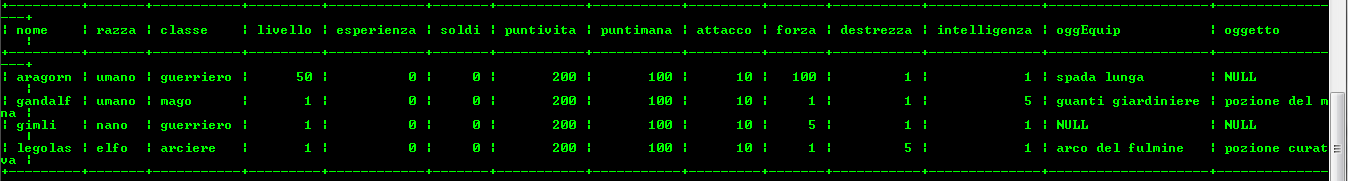
\includegraphics[width=0.7\linewidth]{./immagini/immquery/1-statopersonaggio}
\caption{}
\label{fig:1-statopersonaggio}
\end{figure}

\item Consultazione missioni intraprese da un personaggio (in media 175000 volte al giorno)

\begin{verbatim}
select intraprendenza.personaggio,
 nome as missione,descrizione, livello, completamento,
  ricompensaOro, ricompensaExp,
   ricompensaOgg
from missione join intraprendenzaon 
missione.codMiss= intraprendenza.missione 
where
 personaggio='gandalf';

\end{verbatim}

\begin{figure}[H]
\centering
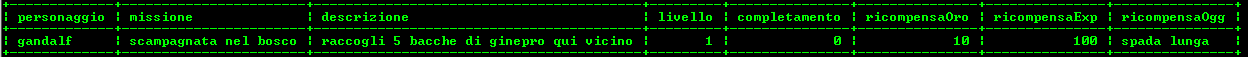
\includegraphics[width=0.7\linewidth]{./immagini/immquery/2-missioniintraprese}
\caption{}
\label{fig:2-missioniintraprese}
\end{figure}

\item Consultazione missioni completate da un personaggio (in media 175000 volte al giorno)

\begin{verbatim}
select completamento.personaggio, nome as missione,
 descrizione, livello, completamento, ricompensaOro,
  ricompensaExp, ricompensaOgg
 
from missione join completamento on missione.codMiss=
 completamento.missione 
where personaggio='Legolas';

\end{verbatim}
\begin{figure}[H]
\centering
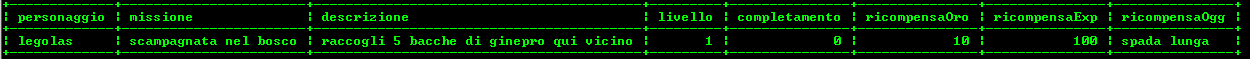
\includegraphics[width=0.7\linewidth]{./immagini/immquery/3-missionicompletate}
\caption{}
\label{fig:3-missionicompletate}
\end{figure}


\item Consultazione abilità apprese da un personaggio(in media 175000 volte al giorno)

\begin{verbatim}
select personaggio.nome as personaggio,
apprendimento.abilità as abilità, abilità.livello, costoMana,
 abilità.attacco,abilità.difesa,abilità.forza,abilità.destrezza,
 abilità.intelligenza from personaggio join apprendimento
 on personaggio.nome= apprendimento.personaggio join
 abilità on apprendimento.abilità = abilità.nome where
 personaggio='legolas';

\end{verbatim}

\begin{figure}[H]
\centering
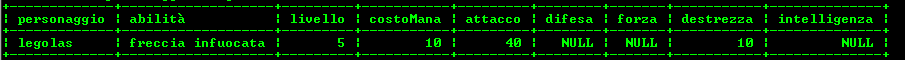
\includegraphics[width=0.7\linewidth]{./immagini/immquery/3-abilitaapprese}
\caption{}
\label{fig:3-abilitaapprese}
\end{figure}


\item Consultazione carrello di un utente(in media 17000 volte al giorno)

\begin{verbatim}

select nomeUt as nome_utente, prodotto.* from carrello
join prodotto on carrello.codPro = prodotto.codPro where
 nomeUt='ginocuoricino';

\end{verbatim}

\begin{figure}[H]
\centering
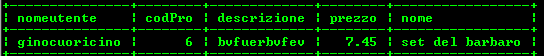
\includegraphics[width=0.7\linewidth]{./immagini/immquery/5-carrelloutente}
\caption{}
\label{fig:5-carrelloutente}
\end{figure}


\item Consultazione prodotti disponibili all'acquisto (in media 35000 volte al giorno)

\begin{verbatim}
select * from prodotto;

\end{verbatim}

\begin{figure}[H]
\centering
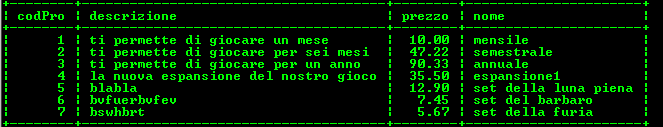
\includegraphics[width=0.7\linewidth]{./immagini/immquery/6-prodottidisponibili}
\caption{}
\label{fig:6-prodottidisponibili}
\end{figure}

\item Consultazione prodotti acquistati da un utente (in media 17000 volte al giorno)

\begin{verbatim}
select nomeUt as nomeutente, prodotto.nome as prodotto,
prodotto.descrizione 
from proprietà join prodotto on proprietà.codPro=prodotto.codPro where 
nomeUt='lollo77';
\end{verbatim}

\begin{figure}[H]
\centering
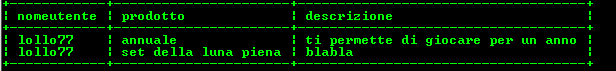
\includegraphics[width=0.7\linewidth]{./immagini/immquery/7-prodottiaquistati}
\caption{}
\label{fig:7-prodottiaquistati}
\end{figure}

\item Consultazione oggetti che un NPC puo vendere (in media 175000 volte al giorno)

\begin{verbatim}
select * from proprietàNPCAmichevole where
 venditore='pino il boscaiolo';

\end{verbatim}
\item Consultazione abilità insegnate da un NPC (in media 175000 volte al giorno)

\begin{verbatim}
select * from insegnamento where maestro='sergente hartman';

\end{verbatim}

\begin{figure}[H]
\centering
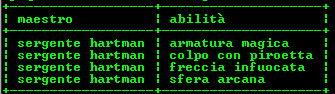
\includegraphics[width=0.7\linewidth]{./immagini/immquery/9-abilitainsegnate}
\caption{}
\label{fig:9-abilitainsegnate}
\end{figure}

\item Consultazione consumabili a tempo attivi di un personaggio (in media 100000 volte al giorno)

\begin{verbatim}
select consumo.*, consumabili.durata from consumo join
 consumabili on consumo.consunto = consumabili.nome
 where consumante ='aragorn';
 
\end{verbatim}

\begin{figure}[H]
\centering
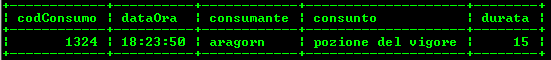
\includegraphics[width=0.7\linewidth]{./immagini/immquery/10-consumati}
\caption{}
\label{fig:10-consumati}
\end{figure}

\end{itemize}
